\documentclass[12pt]{report}
\usepackage[utf8]{inputenc}
\usepackage{graphicx}
\usepackage{titlesec}
\usepackage{xcolor}
\usepackage{fancyhdr}
\usepackage{tikz}
\usepackage{charter}
\usepackage[table]{xcolor} 
\usepackage{float} 
\usepackage{longtable}  
\usepackage{atbegshi} 
\usepackage{array}
\usepackage{hyperref} 
\usepackage{cellspace}
\usepackage[a4paper, left=1in, right=1in, bottom=0.8in, top=0.8in]{geometry}
\usepackage{tikz}
\usepackage{pgf-umlsd}
% Border settings
\newlength{\mymargin}
\setlength{\mymargin}{0.8cm}
\renewcommand{\baselinestretch}{1.4} % 1.5x line height
\pagenumbering{gobble}  % Disables page numbering 
\setlength{\cellspacetoplimit}{6pt}
\setlength{\cellspacebottomlimit}{6pt}
\usetikzlibrary{shapes.geometric, arrows}


\AtBeginShipout{%
  \AtBeginShipoutUpperLeft{%
    \begin{tikzpicture}[remember picture, overlay]
      \draw[line width=0.4pt] 
        ([xshift=\mymargin, yshift=\mymargin] current page.south west) % Bottom-left corner with margin
        rectangle 
        ([xshift=-\mymargin, yshift=-\mymargin] current page.north east); % Top-right corner with margin
    \end{tikzpicture}%
  }%
}

\begin{document}

\newpage

\chapter{\textbf{La Conception d'Application}}
\rule{\linewidth}{1.5pt}


\section*{\textbf{1. Introduction}}

\noindent In this chapter, we present the design phase of our mobile application \textit{Hospital Finder}. Following the analysis and specification of requirements, this stage is essential to define the structural and behavioral aspects of the application. 

\noindent The design phase translates the identified functionalities into technical diagrams that guide implementation. These include use case diagrams, class diagrams, and sequence diagrams. Each diagram offers a different perspective, illustrating how components interact and how the system is structured internally.

\subsection*{1.1 Use Case Actors Overview}

\noindent The application involves multiple actors such as:

\begin{itemize}
    \item \textbf{User}: the main end-user searching for hospitals or clinics.
    \item \textbf{Clinic}: responsible for managing their own clinic profile and associated doctors.
    \item \textbf{Admin}: oversees the system and manages reported data or misuse.
    \item \textbf{Doctor}: while present in the system, the doctor does not interact directly with the application and is managed entirely by the clinic.
\end{itemize}
\newpage
\noindent To better understand the roles and relationships of these actors, we will observe their interactions more thoroughly in the diagrams presented in the following sections. However, \textbf{ a summarized view of the main actors is illustrated in the diagram below: }
\vspace*{0.6cm}
\begin{center}
    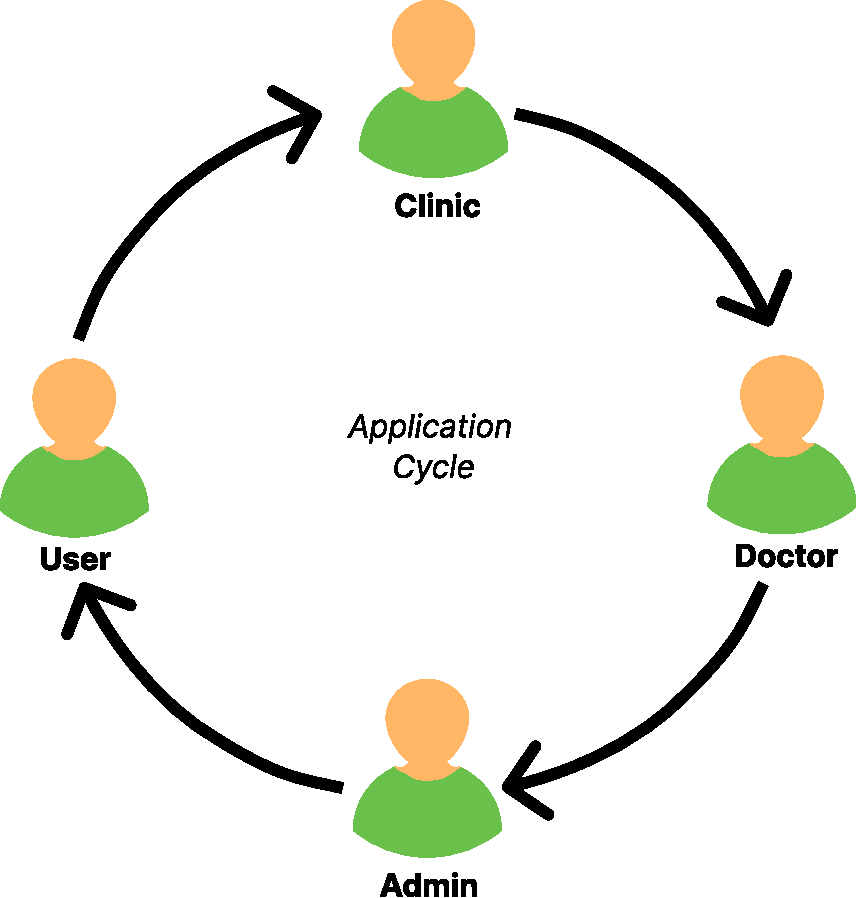
\includegraphics[width=0.7\textwidth]{images/appcucle@2x.pdf}
\end{center}

\section*{2. Detailed Design}

This section presents the core structural design of the \textit{Hospital Finder} application. After analyzing the system’s requirements and actors, we now focus on how these elements are implemented internally.

\noindent The detailed design phase provides a clear technical blueprint by describing the key components, their responsibilities, and how they interact. This allows for a smooth transition from the functional analysis to the actual development.

\noindent UML (Unified Modeling Language) offers various diagrams to describe a software system from different perspectives. These diagrams are generally grouped into two main categories:

\begin{itemize}
    \item \textbf{Structural diagrams} - describe the static aspects of the system, such as classes and their relationships.
    \item \textbf{Behavioral diagrams} - illustrate the dynamic behavior of the system, such as interactions and workflows between components.
\end{itemize}

\begin{center}
    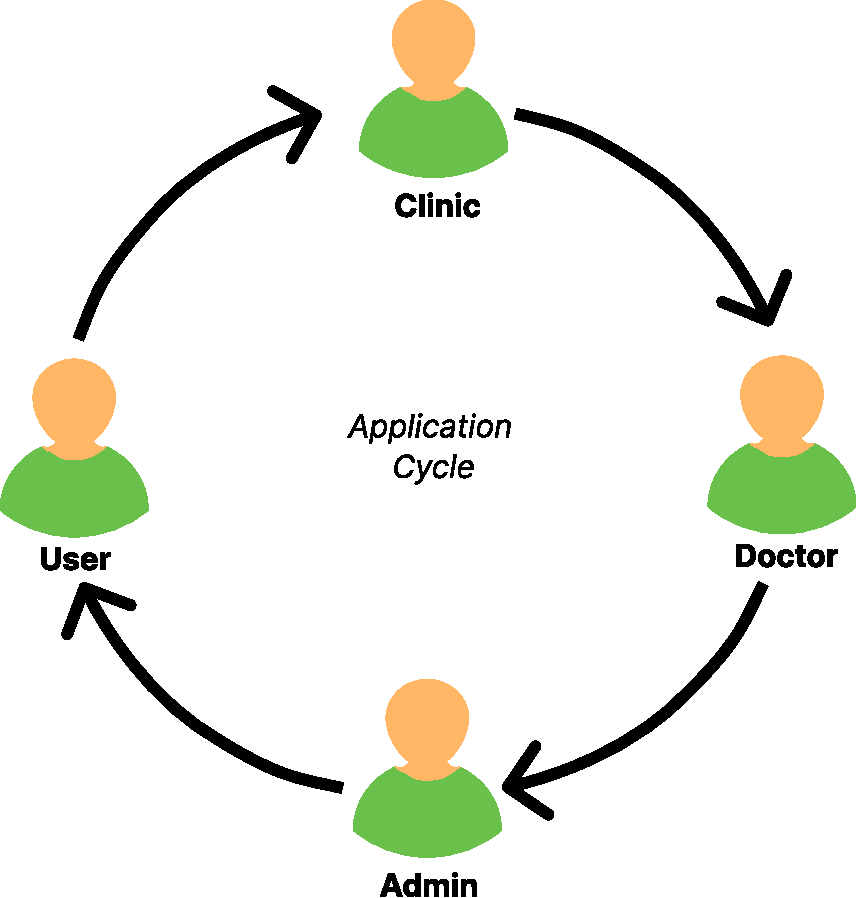
\includegraphics[width=10cm]{images/appcucle@2x.pdf}
\end{center}

\textit{Figure 3.1: Classification of UML diagrams (structure vs behavior).}

\noindent In Chapter 2, we presented a \textbf{Use Case Diagram}, which belongs to the behavioral category. In this chapter, we will explore two additional diagrams:
\begin{itemize}
    \item The \textbf{Class Diagram}, selected from the structural diagrams.
    \item The \textbf{Sequence Diagram}, selected from the behavioral diagrams.
\end{itemize}

These diagrams allow us to model both the architecture and the interactions in our application in a clear and structured manner. We begin with the class diagram in the next section.

\subsection*{2.1 Class Diagram}

A class diagram plays a key role in the object-oriented design of software systems. In this section, we will define what a class diagram is, explain its importance in the development process, and finally present the class diagram of our \textit{Hospital Finder} application.

\subsubsection*{2.1.1 What is a Class Diagram?}

A class diagram is a static structural diagram that describes the types of objects in the system and the various kinds of relationships that exist among them. It shows the system's classes, their attributes, methods, and the associations between objects. It is one of the most commonly used diagrams in UML (Unified Modeling Language) and serves as a blueprint for the implementation phase.

\noindent Each class is represented as a rectangle divided into compartments. The top compartment shows the class name, the middle one lists the attributes, and the bottom lists the operations or methods.

\subsubsection*{2.1.2 Why Use a Class Diagram?}

The class diagram is essential in the software development lifecycle for the following reasons:

\begin{itemize}
    \item It provides a visual overview of the system structure.
    \item It helps developers understand how data is organized and managed.
    \item It facilitates the identification of responsibilities and roles of each class.
    \item It reflects both the logical architecture and the design of the application's database.
    \item It helps in detecting potential design flaws early in the development process.
\end{itemize}

\noindent In the context of our project, the class diagram acts as a bridge between the actors (users, clinics, doctors, and admins) and the data handled internally. It helps clarify how the components of the system interact with one another and ensures a consistent and maintainable code structure.

\subsubsection*{2.1.3 Class Diagram of the Application}

The class diagram of the \textit{Hospital Finder} application was developed based on the functional and non-functional requirements outlined during the analysis phase. It models the following key classes:

\begin{itemize}

    \item \textbf{User}: Represents a normal user of the app who can log in, search for hospitals or clinics, and view details.
    \item \textbf{Clinic}: Can register, log in, and manage doctors under its name.
    \item \textbf{Doctor}: Doctors are managed by clinics and linked to their profiles but do not directly interact with the system.
    \item \textbf{Admin}: Has elevated privileges and can monitor the system, manage content, and respond to reports or user issues.
    \item \textbf{Hospital}: A general entity with details such as name, location, specialty, and contact information.
    \item \textbf{TODO }: TODO LATER 
\end{itemize}

The class diagram is shown below:

\begin{center}
    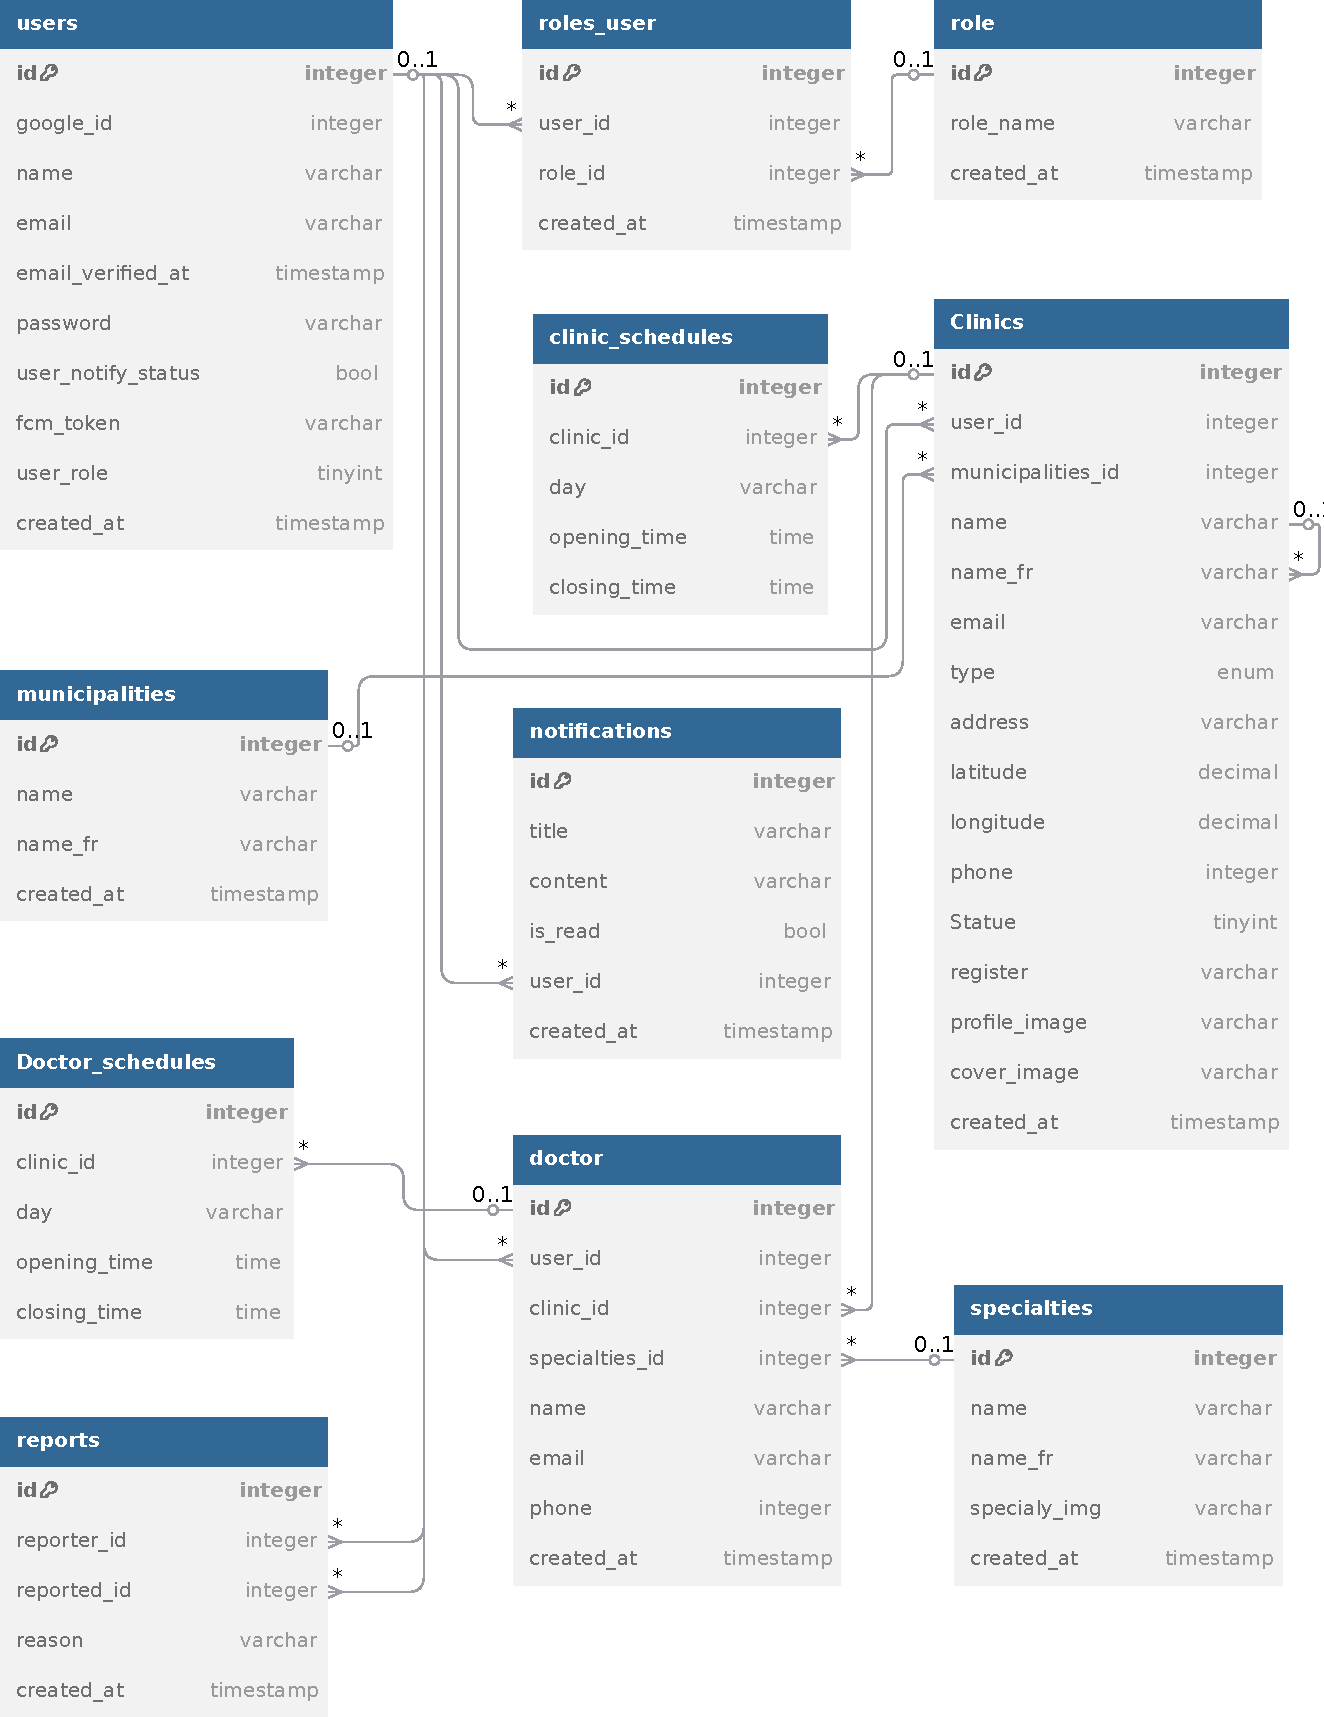
\includegraphics[width=0.95\textwidth]{images/dbclass.pdf}
\end{center}

\textit{Figure 3.2: Class diagram of the Hospital Finder application.}

\subsection*{2.2 Sequence Diagrams}

\subsubsection{2.2.1 Definition}
Sequence diagrams are a type of UML behavioral diagram that show how objects or components in a system interact with each other over time. They describe the flow of messages and the order of operations between actors and system parts in specific scenarios.

Each sequence diagram illustrates how different entities collaborate in a particular process, using lifelines, messages, and activation bars to convey their roles and responsibilities.

\subsubsection*{2.2.2 Purpose and Importance}
Sequence diagrams are essential for modeling dynamic behavior in a system. They help developers understand the exact flow of operations, communication between objects, and timing of events.

In our case, these diagrams allow us to:
\begin{itemize}
    \item Clearly visualize interactions between the application interface, users (like admin), and the backend (database).
    \item Ensure that the designed processes are logically consistent and complete.
    \item Serve as references for both implementation and testing phases.
\end{itemize}

\subsubsection*{2.2.3 Application Sequence Diagrams}
Below, we present a set of sequence diagrams that demonstrate different operations carried out by the admin user. Each diagram focuses on a specific use case and models the message flow involved.

\vspace{1em}

\noindent\underline{\textbf{Admin Managing Specialties and Doctors:}}
This diagram illustrates how the admin adds or updates medical specialties and their associated doctors, including names and photos, through the app interface, with all changes saved to the database.

\begin{sequencediagram}
	% Participants
	\newthread{A}{Admin}
	\newinst[4]{S}{App Interface}
	\newinst[4]{DB}{Database}

	% Login Sequence
	\begin{call}{A}{Login(username, password)}{S}{Authentication Result}
		\begin{call}{S}{Validate Credentials}{DB}{User Data}
		\end{call}
	\end{call}

	% Main Operation
	\begin{call}{A}{Specialty / Doctor Operation}{S}{}
		\begin{sdblock}{alt}{Add or Edit?}
			% Add Specialty Path
			\begin{sdblock}{Add Specialty / Doctor}{}
				\begin{call}{S}{Create Specialty Entry}{DB}{Success}
				\end{call}
				\begin{call}{A}{Update Specialty / Doctor Name}{S}{Confirmation}
					\begin{call}{S}{Store Name}{DB}{Success}
					\end{call}
				\end{call}
				\begin{call}{A}{Update Specialty / Doctor Photo}{S}{Confirmation}
					\begin{call}{S}{Store Photo}{DB}{Success}
					\end{call}
				\end{call}
			\end{sdblock}

			% Edit Specialty Path
			\begin{sdblock}{Edit Specialty / Doctor}{}
				\begin{call}{A}{Enter New Name}{S}{Confirmation}
					\begin{call}{S}{Update Name}{DB}{Success}
					\end{call}
				\end{call}
				\begin{call}{A}{Upload New Photo}{S}{Confirmation}
					\begin{call}{S}{Update Photo}{DB}{Success}
					\end{call}
				\end{call}
				\begin{call}{A}{Save Changes}{S}{Confirmation}
					\begin{call}{S}{Commit Changes}{DB}{Success}
					\end{call}
				\end{call}
			\end{sdblock}
		\end{sdblock}

		% Final Operations
		\begin{call}{S}{Finalize Operation}{DB}{Success}
		\end{call}
	\end{call}

	% Final Response
	\mess{S}{Operation Complete}{A}
\end{sequencediagram}

\noindent\underline{\textbf{Admin Managing Terms and Conditions of the App:}}
This sequence diagram models how the admin adds or edits the Terms and Conditions of the application. Admin actions pass through the interface, updating the data in the database accordingly.

\vspace*{1em}

\begin{sequencediagram}
	% Participants with increased spacing
	\newinst[3]{A}{Admin}
	\newinst[3]{S}{App Interface}
	\newinst[3]{DB}{Database}

	% Vertical space before operations
	\postlevel
	\vspace{0.5cm}
	\prelevel

	% Main Operation
	\begin{call}{A}{Terms Operation}{S}{}
		\begin{sdblock}{alt}{Edit or Add?}
			% Edit Terms Path
			\begin{sdblock}{Edit Terms}{}
				\begin{call}{A}{Modification of Terms}{S}{Confirmation}
					\begin{call}{S}{Update Terms}{DB}{Success}
					\end{call}
				\end{call}
				\begin{call}{A}{Save Changes}{S}{Confirmation}
					\begin{call}{S}{Commit Changes}{DB}{Success}
					\end{call}
				\end{call}
			\end{sdblock}

			% Add Terms Path
			\begin{sdblock}{Add Terms}{}
				\begin{call}{A}{Enter Terms Information}{S}{Confirmation}
					\begin{call}{S}{Create New Terms}{DB}{Success}
					\end{call}
				\end{call}
				\begin{call}{A}{Save}{S}{Confirmation}
					\begin{call}{S}{Finalize Terms}{DB}{Success}
					\end{call}
				\end{call}
			\end{sdblock}
		\end{sdblock}

	\end{call}

	\mess{S}{Operation Complete}{A}
\end{sequencediagram}

\noindent\underline{\textbf{Searching for a Clinic or Doctor:}}
This sequence diagram models the process in which the user searches for a clinic or doctor. The user logs into the app, performs a search, and the app displays results or error messages if the search does not yield results.

\vspace*{1em}

\begin{sequencediagram}
	% Participants with increased spacing
	\newinst[3]{U}{User}
	\newinst[3]{S}{App Interface}
	\newinst[3]{DB}{Database}

	% Login and Initial Search
	\begin{call}{U}{Login(username, password)}{S}{}
		\begin{call}{S}{Validate Credentials}{DB}{Result}
		\end{call}
		\begin{sdblock}{alt}{Are credentials valid?}
			\begin{sdblock}{option}{Yes}
				\mess{S}{Login Success}{U}
			\end{sdblock}
			\begin{sdblock}{option}{No}
				\mess{S}{Login Failed or Search as Guest}{U}
			\end{sdblock}
		\end{sdblock}
	\end{call}

	\postlevel
	\vspace{0.5cm}
	\prelevel

	% Search Loop
	\begin{sdblock}{loop}{Until valid clinic/doctor found}
		\begin{call}{U}{Enter Clinic/Doctor Name}{S}{}
		\end{call}

		\begin{call}{S}{Search Records}{DB}{Search Results}
		\end{call}

		\begin{sdblock}{alt}{Found?}
			% Found case
			\begin{sdblock}{Yes}{}
				\begin{call}{S}{Display Results}{U}{}
				\end{call}
			\end{sdblock}

			% Not found case
			\begin{sdblock}{No}{}
				\begin{call}{S}{Show "Not Found" Error}{U}{}
				\end{call}
				\begin{call}{U}{Retry Search}{S}{}
				\end{call}
			\end{sdblock}
		\end{sdblock}
	\end{sdblock}
	% Final Results
	\begin{call}{S}{Display Final Results}{U}{}
	\end{call}
\end{sequencediagram}

\vspace*{1em}

\noindent\underline{\textbf{Clinic Registering In The Application :}}
This sequence diagram illustrates the process by which a clinic registers on the app. The clinic submits information through the app, which is then stored in the database. Admin verifies the submission and either approves or rejects the registration.

\vspace*{1em}

\begin{sequencediagram}
	% Participants with increased spacing
	\newinst[2]{C}{Clinic/Doctor}
	\newinst[1.5]{A}{App Interface}
	\newinst[1.5]{DB}{Database}
	\newinst[2]{Ad}{Admin}

	% Registration Flow
	\begin{call}{C}{Submit Information}{A}{}
		\begin{call}{A}{Store Information}{DB}{Storage Result}
		\end{call}
		\mess{A}{Submission Received}{C}
	\end{call}

	% Admin Verification
	\postlevel
	\vspace{1cm}
	\prelevel

	\begin{call}{DB}{Check Pending Requests}{Ad}{Registration Data}
	\end{call}

	\begin{sdblock}{Alternative}{Admin Decision}
		\begin{sdblock}{Acceptance}{}
			\begin{call}{DB}{Approve Account}{Ad}{}
			\end{call}
			\mess{Ad}{Send Approval}{A}
			\mess{A}{Account Approved}{C}
		\end{sdblock}

		\begin{sdblock}{Refusal}{}
			\begin{call}{DB}{Reject Application}{Ad}{}
			\end{call}
			\mess{Ad}{Send Rejection}{A}
			\mess{A}{Account Rejected}{C}
		\end{sdblock}
	\end{sdblock}

	% Login After Approval
	\postlevel
	\vspace{1cm}
	\prelevel

	\begin{sdblock}{Optional}{If Approved}
		\begin{call}{C}{Login}{A}{}
			\begin{call}{A}{Verify Credentials}{DB}{}
			\end{call}
			\begin{call}{A}{Grant Access}{C}{}
			\end{call}
		\end{call}
	\end{sdblock}
\end{sequencediagram}

\noindent\underline{\textbf{Admin Managing Clinics Requests:}}
This sequence diagram models the process by which the admin handles clinic registration requests. The admin reviews the applications, makes a decision, and updates the database accordingly.

\vspace*{1em}

\begin{sequencediagram}
	% Participants with increased spacing
	\newinst[2]{Ad}{Admin}
	\newinst[3]{A}{App Interface}
	\newinst[3]{DB}{Database}

	% Access Requests List
	\begin{call}{Ad}{Access Request List}{A}{}
		\begin{call}{A}{Fetch Pending Requests}{DB}{Requests Data}
		\end{call}
	\end{call}

	% Review Process
	\postlevel
	\vspace{0.5cm}
	\prelevel

	\begin{sdblock}{Loop}{For each application}
		\begin{call}{Ad}{Select Application}{A}{}
		\end{call}

		\begin{call}{Ad}{Review Details}{A}{}
			\begin{call}{A}{Get Full Application}{DB}{Complete Data}
			\end{call}
		\end{call}

		\begin{sdblock}{Alternative}{Decision}
			\begin{sdblock}{Acceptance}{}
				\begin{call}{Ad}{Confirm Approval}{A}{}
					\begin{call}{A}{Update Status}{DB}{Approved}
					\end{call}
				\end{call}
				\mess{DB}{Approval Notification}{Ad}  % To notify clinic
			\end{sdblock}

			\begin{sdblock}{Refusal}{}
				\begin{call}{Ad}{Confirm Rejection}{A}{}
					\begin{call}{A}{Update Status}{DB}{Rejected}
					\end{call}
				\end{call}
				\mess{DB}{Rejection Notification}{Ad}  % To notify clinic
			\end{sdblock}
		\end{sdblock}
	\end{sdblock}

	% Completion
	\postlevel
	\vspace{0.5cm}
	\prelevel
	\mess{A}{Processing Complete}{Ad}
\end{sequencediagram}

\vspace*{1em}

\noindent\underline{\textbf{User Report Activity:}}
This sequence diagram models the process when a user submits a report. After submission, the admin reviews the report and takes action, which may result in a notification being sent to the user.

\vspace*{1em}

\begin{sequencediagram}
	% Participants with increased spacing
	\newinst[1.5]{U}{User}
	\newinst[2]{A}{App Interface}
	\newinst[1.5]{DB}{Database}
	\newinst[1.5]{Ad}{Admin}

	% Reporting Flow
	\begin{call}{U}{Submit Report}{A}{}
		\begin{call}{A}{Store Report}{DB}{Confirmation}
		\end{call}
		\mess{A}{Report Submitted notification}{U}
	\end{call}

	% Admin Review Process
	\postlevel
	\vspace{0.5cm}
	\prelevel

	\begin{call}{Ad}{Check New Reports}{DB}{Report Data}
	\end{call}

	\begin{sdblock}{Alternative}{Report Validation}
		\begin{sdblock}{Valid Report}{}
			\begin{call}{Ad}{Restrict Clinic}{DB}{}
				\begin{call}{DB}{Update Status}{DB}{Restricted}
				\end{call}
			\end{call}
			\mess{Ad}{Notify Action Taken}{A}
		\end{sdblock}

		\begin{sdblock}{False Report}{}
			\begin{call}{Ad}{Mark as False}{DB}{}
			\end{call}
			\mess{Ad}{Ignore Report}{A}
		\end{sdblock}
	\end{sdblock}

	% Notification
	\postlevel
	\vspace{0.5cm}
	\prelevel
	\mess{DB}{Status Updated}{A}
\end{sequencediagram}



\section*{3. Conclusion}

\vspace{1em}

\noindent
The design phase of our \textit{Hospital Finder} mobile application has been carefully structured to ensure clarity, consistency, and extensibility. Throughout this chapter, we laid the foundation of the application by modeling its components and interactions using essential UML diagrams.

\vspace{1em}

\noindent
We began with the class diagram, which defined the main entities such as users, clinics, doctors, and the admin, along with their relationships. This provided a blueprint for structuring the database and guiding the backend development. Each class was tailored to support the application's functionality, ensuring that both user and system needs are represented.

\vspace{1em}

\noindent
Subsequently, we introduced a series of sequence diagrams to illustrate the dynamic behavior of the system. These diagrams covered key interactions including user registration, clinic requests, login, searching, and admin management operations. Particular focus was placed on administrator features—such as reviewing clinic applications, editing terms and conditions, and handling user reports—emphasizing the application's flexibility and administrative control.

\vspace{1em}

\noindent
Each interaction was modeled to ensure that data flows seamlessly through the app interface and is consistently stored or retrieved from the database. The logical flow within these diagrams also helps in pinpointing edge cases, user roles, and error-handling scenarios.

\vspace{1em}

\noindent
In summary, this conception phase has transformed abstract requirements into detailed structural and behavioral models. These models not only support the system’s current requirements but also anticipate future enhancements. The groundwork laid here will facilitate a smoother transition to the implementation phase, ensuring that development is aligned with the overall system design.








\end{document}
